\documentclass[article]{beamer}
\usetheme{Warsaw}
\setbeamertemplate{footline}[frame number]

\usefonttheme[]{serif}
\usepackage{amsmath, latexsym, color, graphicx, amssymb, bm, here}
\usepackage{epsf, epsfig, pifont,tikz,subfigure}
\usepackage{graphics, calrsfs}
\usepackage{times}
\usepackage{fancybox,calc}
\usepackage{palatino,mathpazo}
\usepackage{amsfonts}
\usepackage{sidecap}
\usepackage{listings}
\usepackage{hyperref}

\title{Dynamic Programming}
\author{David Jacobo \\ \href{mailto:jguillen@cimat.mx}{jguillen@cimat.mx}}
\date{\scriptsize{\today}}

\AtBeginSection[]
{
  \begin{frame}{Outline}
    \tableofcontents[currentsection]
  \end{frame}
}

\begin{document}

%%%%%%%%%%%%%%%%%%%%%%%%%%%%%%
\maketitle

%%%%%%%%%%%%%%%%%%%%%%%%%%%%%%
\begin{frame}
\begin{block}{Dynamic Programming (DP):}
	Also called \textbf{'memoization'} is a paradigm focused on solving \textbf{optimization 
	problems}. For a problem to be solved with DP, it must exhibit an \textbf{optimal substructure and
	overlapping sub-problems}.
	
	\vspace{8mm}
	
	A critical part on designing DP solutions boils down to recognizing/defining the 
	required \textbf{state and transitions}. There are two typical ways to express a DP solution: \textbf{bottom up and top down}.
\end{block}
\end{frame}

%%%%%%%%%%%%%%%%%%%%%%%%%%%%%%

\section{Basics}

\subsection{Motivation}
\begin{frame}
	\frametitle{Motivation: Fibonacci series}
	Figure 1: Recursion tree with and without DP
	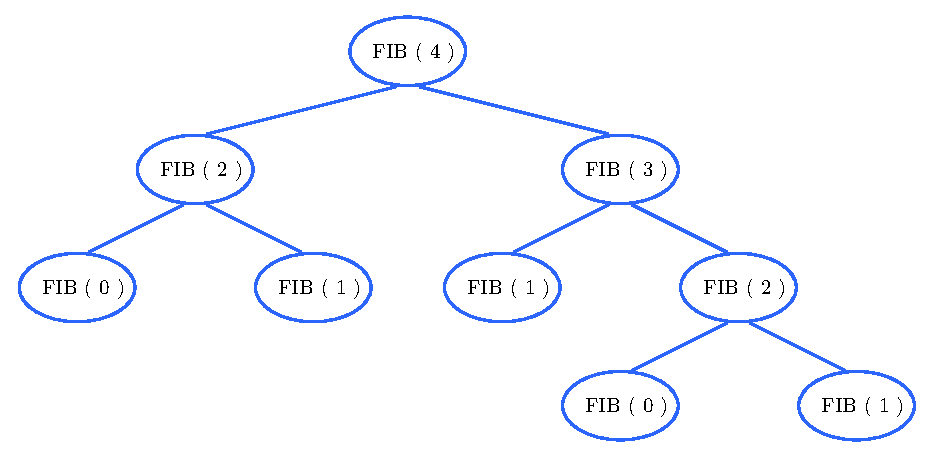
\includegraphics[scale=0.5]{./figures/fib.eps}
\end{frame}

\subsection{Properties}
\begin{frame}
	\frametitle{Optimal substructure}
	Refers to the fact that you need to know the optimal solution for smaller instances of the same problem in order to expand your solution to the required size.
	
	\vspace{8mm}
	
	Insert images of shortest paths	
\end{frame}

\begin{frame}
	\frametitle{Overlapping sub-problems}
	This property becomes evident when you are drawing a recurrence tree, whenever you are calling the exact instance of the problem 2 or more times it's clear than an overlap exists.
	
	\vspace{8mm}
	
	Insert fibonacci recurrence tree or the coin change one.	
\end{frame}

\begin{frame}
	\begin{block}{State:}
		A state is the list of parameters which represent each sub-problem in a unique way. Expand this !!!
	\end{block}
\end{frame}

\begin{frame}
	\begin{block}{Transition:}
		A transition defines if two states have a direct relation or not. Pls expand !!
	\end{block}
\end{frame}

\section{Design and coding styles}

\subsection{Bottom up}
\begin{frame}
	\frametitle{Bottom up}
	This variant solves and store the solutions for \textbf{all the smaller instances} before solving the bigger instance (which is the one that matters for us).
	
	\vspace{8mm}
	
	Figure: Need a table where computation can be seen
\end{frame}

\subsection{Top down}
\begin{frame}
	\frametitle{Top down}
	The top down approach relies in calling only the instances which are really needed for the given problem.
\end{frame}

\subsection{Fight!}
\begin{frame}
	\frametitle{So, which one is better?}
	Remember that both are based on the same recurrence formula, thus they are equaly correct.
\end{frame}

\section{Algorithm analysis}

\subsection{Time complexity}
\begin{frame}
	\frametitle{Time complexity}
	Time complexity refers to the amount of time it will take to your algorithm to finish in terms of a given input. 
	
	\vspace{8mm}	
	
	\textbf{O(number of different states * time to solve each state)}
\end{frame}

\subsection{Space complexity}
\begin{frame}
	\frametitle{Space complexity}
	The space complexity refers to the amount of memory necessary to store all the answers, so it basically express how many cells your array has.
	
	\vspace{8mm}
	
	\textbf{O(dimensions of the array)}
\end{frame}

\section{Classic problems}
\begin{frame}
	Counting problems, cost-gain problems (knapsack?)
\end{frame}

\section{Pro-tips}
\begin{frame}
	\frametitle{Pro-tips}
	\begin{itemize}
		\item Study the theory.
		\item Write solutions for the classic problems.
		\item Try out both variants.
		\item ??
		\item Profit.
	\end{itemize}
	
	\vspace{5mm}
	
	It is also worthy to explore the \textbf{sliding window} trick in order to save memory, or selecting a \textbf{different data structure} for saving the intermediate states specially when using the top-down approach. \textbf{DP is a trade-off between space and time!}
\end{frame}

%%%%%%%%%%%%%%%%%%%%%%%%%%%%%%
\begin{frame}[plain]
\frametitle{}
\begin{center}
\Huge{\color{blue}{Q \& A}}
\end{center}
\end{frame}

%%%%%%%%%%%%%%%%%%%%%%%%%%%%%%%%
\begin{frame}[plain]
	\textbf{References}
	\begin{itemize}
		\item \href{https://sites.google.com/site/stevenhalim/}{Competitive Programming site}
		\item \href{https://github.com/davidjacobo/algorists/}{Algorists' repository}
	\end{itemize}
\end{frame}
\end{document}